\documentclass[12pt, a4paper]{article}
\usepackage{graphicx}
\usepackage{amsmath}
\usepackage{natbib}
\usepackage[utf8]{inputenc}    
\usepackage{natbib}
\usepackage{float}
\usepackage[usenames,dvipsnames]{xcolor}
\usepackage[left=2cm,right=2cm,top=2cm,bottom=2cm]{geometry}
\usepackage{setspace}
\usepackage{listings}
\doublespacing

\begin{document}
\title{A look into binding site lengths for SOX-family transcription factors in the telomeric region of H.sapiens chromosome 1}
\author{Debduth Bardhan Pijush}
\date{May 8th, 2017}
\maketitle

\section{Introduction}
A transcription factor is a protein that acts as regulatory element used for gene expression, acting as a signal activating or deactivating a gene for transcription. Once the gene is transcribed into RNA, it is ready to be processed for protein production. Protein is the structural element of all life so understanding how and why transcription occurs is important to understanding the mechanisms of the growth of life. The sites on the chromosomes where these transcription factors bind is called binding sites. These binding sites are located in the promoter region of a chromosome as short DNA sequences, and are prone to evolutionary change, observed by the divergence in binding sites of yeast structural protein regulators \cite{evolution}. These binding sites however are not always identical, and have different frequencies in the sequence, and as a result any object representing the transcription factor binding sites must include for this variation.\newline

Each of these chromosomes have telomeres on its two ends to prevent the chromosome from fusing with other chromosomes and to prevent damage to the sequence. It consists of a repeating sequence of nucleotides, which is TTAGGG for verterbrates. For \textit{H.sapiens}, this repeated sequence can expand into 11 kb (kilobases) at birth, however it decreases over time during cell division and in certain situations can extend as well. Because of the high levels of activity in this region, in terms of insertion and deletion, it is possible that the transcription factor binding sites in this region might be smaller in order to decrease the probability of alteration of its binding site. Telomerase is the enzyme that is able to reverse the process of the shortening telomeres, which is heavily expressed in embryonic stem cells so it can divide repeatedly. The transcription factor Sox2 is protein that regulates the pluripotency of cells, the ability to form all kinds of cell types, and is shown that when it causes a reprogramming of somatic cells into a pluripotent state, it occurs alongside telomerase activation and telomere length extension \cite{telomere}. This shows that there is a link between Sox2 and telomeres. This warrants looking into the Sox-family transcription factors, all of which are responsible for cell fate decisions and development of organisms, and correlating its proximity to the telomeric region, to see if the length of the transcription factor binding sites are affected by the tumultuous state of the telomeric region in its insertions and deletions.
\section{Methods}
The libraries MotifDb, MotIV, seqLogo, Biostrings, and BSgenome.Hsapiens.UCSC.hg19 were used. First, the data was extracted with the genome being extracted from the UCSC database and the Sox-motifs extracted from the MotifDb database from the jolma2013 data source. A sequence logo for Sox9 is shown below, showing the probabilistic nature of the transcription factor binding site. 
\begin{figure}[H]
\caption{Sequence Logo for Sox9}
\centering
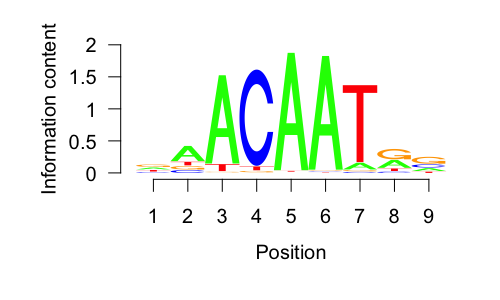
\includegraphics[width=\textwidth]{seqlogo.png}
\end{figure}
The MotifDb gives the position frequency matrix, but using the matchPWM command, the PFM is converted into a position weight matrix with the genome's chromosome 1 is used as a background and matched accordingly for the positions on the chromosome. The information about each Sox-family transcription factor's binding sites on chromosome 1 of the human genome is stored, and then graphed as a frequency distribution. This plot explains to us the general locations of the transcription factor which can then be analyzed further whether there are shorter transcription factor binding sites in the telomeric regions at both ends of the chromosome. A sample of the Sox-family transcription factor binding sites are selected as short-length binding sites, which are Sox9 of length 9 and Sox14 of length 12, and long-length binding sites, which are Sox2 of length 17, Sox7 of length 16, and Sox8 of length 16. These transcription factors were binned to give two conglomerate histograms depicting the frequency distributions over the start sites of the binding sites on the chromosome. To test for significance, a linear model was fit from each end of each chromosome to the binding site prevalence peak, right before the centromere point since there are no binding sites in that region and it would sway the results. ANOVA was done with both ends of the chromosome between the short-length frequency and long-length frequency, to test for significance of the conclusion.

\section{Results}
The results of the position frequency distribution of the short-length Sox-family binding sites and the long-length transcription factor binding sites actually did not come out as expected. In both circumstances of binding site lengths, there were less binding sites on the ends of the chromosomes, in the telomeric region, than the center. However, in the comparison between the short-length and long-length binding sites, one side of the small-length binding site slope was significantly different than both the same side and the other side of the chromosome for the long-length binding site slope, with p-values of 1.622e-5. The absolute value of the slope (since one pairing is on opposite sides) showed that the slope of the small-length binding site's slope in the "front" end was significantly greater than the slope of the long-length binding site's slope in both ends. This indicates that there is a greater decrease in binding sites in the "front" region than the middle region of the chromosome of the short-length transcription factor binding sites, as compared to the long-length transcription factor binding sites. The frequency distributions of both lengths of Sox-family binding sites on human chromosome 1 are shown below
\begin{figure}[H]
\caption{The frequency distribution of where on the chromosome the longer-length transcription factor binds}
\centering
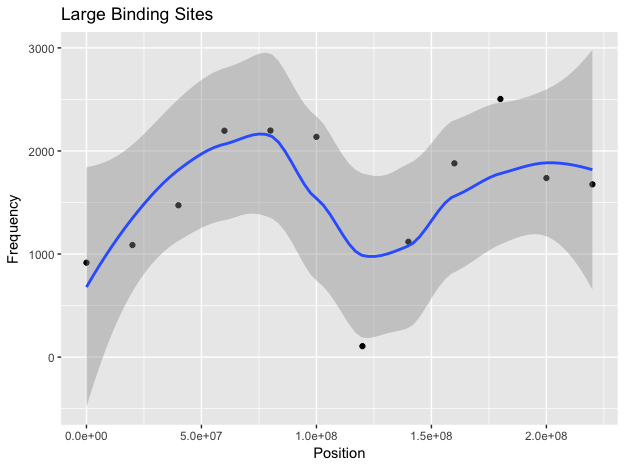
\includegraphics[width=\textwidth]{largebsplot.png}
\end{figure}
\begin{figure}[H]
\caption{The frequency distribution of where on the chromosome the shorter-length transcription factors bind}
\centering
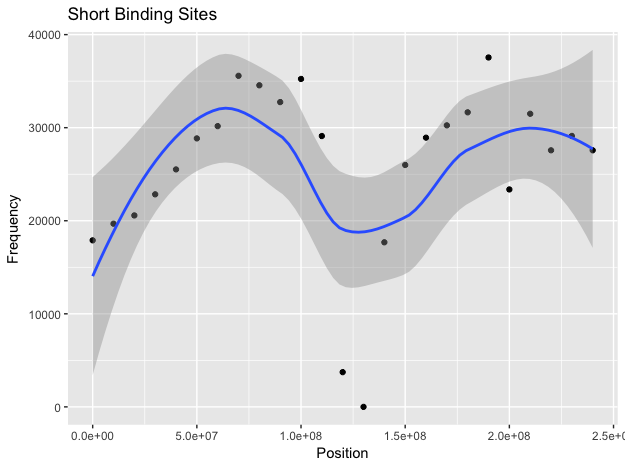
\includegraphics[width=\textwidth]{shortbsplot.png}
\end{figure}
\section{Conclusion}
Through the results, it can be said that there is no significant increase in short-length Sox-family binding sites near the telomeric regions of human chromosome 1, as compared to the long-length Sox-family binding sites. The results actually said otherwise to what was expected as there were considerably less binding sites near the telomeric region proportionate to the rest of the chromosome for the short-length binding sites, as compared to the long-length binding sites. This might be because of the inherent nature of the Sox-family transcription factors on human chromosome 1, a small sample size of the Sox-family transcription factors, or an error in data collection and analysis. Either way, this significant relationship for the short-length binding sites calls for further looks into the relationships between transcription factor binding site lengths and chromosomal position.
\section{Appendix of Code}

\begin{lstlisting}[language=R]
library(MotifDb)
library(MotIV)
library(seqLogo)
library(motifStack)
library(Biostrings)
library(GenomicFeatures)
library(org.Sc.sgd.db)
library(BSgenome.Hsapiens.UCSC.hg19)
library(ggplot2)

#Gather Data
genome = BSgenome.Hsapiens.UCSC.hg19
sox = query(query(query(MotifDb,'sapien'),'Sox'),'jolma')
soxx=c(sox[1],sox[2],sox[7],sox[10],sox[13],sox[16],sox[20],sox[27],sox[30])
unlist(soxx)
seqLogo(as.list(soxx)[[1]])

#Transcription Factors PWM
sox9 = (matchPWM(unlist(soxx[1]),genome$chr1)) #9
sox10 = (matchPWM(unlist(soxx[2]),genome$chr1)) #15
sox14 = (matchPWM(unlist(soxx[3]),genome$chr1)) #12
sox15 = (matchPWM(unlist(soxx[4]),genome$chr1)) #15
sox18 = (matchPWM(unlist(soxx[5]),genome$chr1)) #15
sox21 = (matchPWM(unlist(soxx[6]),genome$chr1)) #15
sox2 = (matchPWM(unlist(soxx[7]),genome$chr1)) #17
sox7 = (matchPWM(unlist(soxx[8]),genome$chr1)) #16
sox8 = (matchPWM(unlist(soxx[9]),genome$chr1)) #16

#Short Binding Sites
smallbs = c(start(sox9),start(sox14))
hist(smallbs)
plot(density(smallbs))
head(smallbs)
tail(smallbs)
smallbins = seq(0,2.5*10^8,by=1*10^7)
smallbins = smallbins[1:25]
smallbs.cut = cut(smallbs,smallbins,right=FALSE)
a = table(smallbs.cut)
freqsmallbs = c(17895,19682,20572,22840,25517,28849,30167,35574,34555,32751,35236,29104,3732,0,17685,25993,28926,30252,31651,37543,23364,31494,27571,29111,27572)
plot(smallbins,freqsmallbs)
smallmodel <- lm(freqsmallbs ~ poly(smallbsmallins,2))
#predsmall = smallmodel$coefficients[1]+smallmodel$coefficients[2]*smallbins+smallmodel$coefficients[3]*smallbins^2
#points(smallbins, predict(smallmodel), type="l", col="red", lwd=2)
dfsmall = data.frame(Position=smallbins,Frequency=freqsmallbs)
smallplot = ggplot(dfsmall,aes(x=Position,y=Frequency))+geom_point()+geom_smooth()+labs(title="Short Binding Sites")
dfsmallfront = data.frame(Position=smallbins[1:8],Frequency=freqsmallbs[1:8])
smallfrontmodel = lm(dfsmallfront$Frequency~dfsmallfront$Position)
dfsmallback = data.frame(Position=smallbins[20:25],Frequency=freqsmallbs[20:25])
smallbackmodel = lm(dfsmallback$Frequency~dfsmallback$Position)

#Long Binding Sites
largebs = c(start(sox2),start(sox7),start(sox8))
hist(largebs)
head(largebs)
tail(largebs)
plot(density(largebs))
largebins = seq(0,2.5*10^8,by=2*10^7)
largebins = largebins[1:12]
largebs.cut = cut(largebs,largebins,right=FALSE)
b = table(largebs.cut)                                                                                       
freqlargebs = c(916,1087,1473,2196,2198,2137,106,1119,1880,2504,1737,1676)
dflarge = data.frame(Position=largebins,Frequency=freqlargebs)
largeplot = ggplot(dflarge,aes(x=Position,y=Frequency))+geom_point()+geom_smooth()+labs(title="Large Binding Sites")
dflargefront = data.frame(Position=largebins[1:5],Frequency=freqlargebs[1:5])
largefrontmodel = lm(dflargefront$Frequency~dflargefront$Position)
dflargeback = data.frame(Position=largebins[10:12],Frequency=freqlargebs[10:12])
largebackmodel = lm(dflargeback$Frequency~dflargeback$Position)

#Analyze
anova(smallbackmodel,largebackmodel)
anova(smallfrontmodel,largefrontmodel) #significant
anova(smallfrontmodel,largebackmodel) #significant
anova(smallbackmodel,largefrontmodel)
\end{lstlisting}
\bibliographystyle{plain}
\bibliography{bibby}
\end{document}